\documentclass{article}
\usepackage{amsmath,amssymb}
\usepackage{caption}
\usepackage{graphicx}
\usepackage{url}

\def\N{{\mathcal{N}}}
\def\NN{{\mathbb{N}}}
\def\ZZ{{\mathbb{Z}}}
\def\RR{{\mathbb{R}}}
\def\un{{\rm{1\!\!1}}}
\def\CC{{\mathcal{C}}}
\def\HH{{\mathcal{H}}}
\def\UU{{\mathcal{U}}}
\def\II{{\mathcal{I}}}
\def\JJ{{\mathcal{J}}}
\def\TT{{\mathcal{T}}}
\def\PP{{\mathcal{P}}}
\def\SS{{\mathcal{S}}}
\def\WW{{\mathcal{W}}}
\def\KK{{\mathcal{K}}}
\def\MM{{\mathcal{M}}}
\def\YY{{\mathcal{Y}}}
\def\VV{{\mathcal{V}}}

\newtheorem{mydef}{Definition}
% \newtheorem{theorem}{Theorem}
% \newtheorem{lemma}{Lemma}
 \newtheorem{prop}{Proposition}
 \newtheorem{conj}{Conjecture}


\title{Report of Final Project of ML, Out-of-Domain PoS tagging}
\author{Xinneng XU et Wei HUANG}
\begin{document}
\maketitle

\begin{abstract}
The goal of this project is to design a PoS tagging which can well solve the problem of Out-of-Domain PoS tagging. And evaluate this PoS tagging on the different combination of train and test sets by considering: 1.its precision over the whole test set, 2.this precision over the ambiguous words, 3.its precision on Out-of-Vocabulary(OOV) words.For now, the PoS tagger we designed gives a 95.53\% accuracy on all the test dataset of corpus 'fr.ftb'. Finally, we implement and evaluate the different classifiers HMM Tagging which gives a 94.63\% accuracy.
\end{abstract}

\noindent{\textbf{Keywords}:
Part-of-Speech; Out-of-Domain PoS tagging; Machine Learning; NLP; Classifier; HMM }

\section{Introduction}
In traditional grammar, a PoS is a category of words which have similar grammatical properties. PoS tagging can be considered as a multi-class classification problem, and with very simple features achieve human-comparable performance. However, the PoS tagger performance decrease with the increasing of the percentage of sentences that depart from training dataset. We aim to evaluate the impact of changes in domain and develop the features and models that are robust to changes in domain.

In this report we describe a little about the different french corpus we used in our work in the difference of the size of the train and test sets, the differences between UGC corpora (denoted as 'in-domain' in the following) and 'canonical' corpora (denoted as 'out-domain' in the following) etc. Then we describe the Perceptron, a part-of-speech (POS) tagger which uses the principal notion of Multi-Classification and the classical Hidden Markov Model (HMM) tagger which is described in \cite{charniak1993equations}. After that we describe the features we extracted from the corpus, such as the suffix of the token, the shape features. Finally we show the evaluations of the different classifiers and describe the results obtained from our experiments.


\section{Experimental French Corpus}
In this section, we describe the similarity between different datasets and the differences of the train and test sets.

There are 6 different corpus in our sources : 1.fr.ftb, 2.fr.gsd, 3.fr.partut, 4.fr.pud, 5.fr.sequoia, 6.fr.spoken. These corpus come from $Universal Dependencies 2.3$ project \cite{nivre2017universal}. 

\subsection{The resource}
As marked briefly in Table \ref{table_resource}, $(1) fr.pud$  is a treebank of sentences from the newspaper Le Monde, initially manually annotated with morphological information and phrase-structure and then converted to the Universal Dependencies annotation scheme. $(2) fr.gsd$ contains many truncated sentences (date missing for instance). Almost every truncated sentence is from Wikipedia. $(3) fr.partut$ is a conversion of a multilingual parallel treebank developed at the University of Turin, and consisting of a variety of text genres, including talks, legal texts and Wikipedia articles, among others. $(4) pud$ is created for the [CoNLL 2017 shared task on Multilingual Parsing from Raw Text to Universal Dependencies](http://universaldependencies.org/conll17/). $(5) fr.sequoia$ is an automatic conversion of the Sequoia Treebank corpus [French Sequoia corpus](http://deep-sequoia.inria.fr). $(6) fr.spoken$ is a Universal Dependencies corpus for spoken French.

\begin{table}[h]
\caption{The resource of Corpus}
\vspace{5pt}
\centering
    
\begin{tabular}{|l|l|}
\hline
Corpus & Resource\\
\hline
fr.ftb     & news \\
fr.gsd     & blog news reviews wiki\\
fr.partut  & legal news wiki\\
fr.pud     & news wiki\\
fr.sequoia & medical news notification wiki\\
fr.spoken  & spoken \\
\hline
\end{tabular}
\label{table_resource}
\end{table}


\subsection{Size of Corpus} 
Table 1 shows the size (number of sentences and words) of the difference of the train and test set, in which the number of sentences and words in corpus 'fr.ftb' is the largest, 14759 and 44228 respectively in train\_set. 

\begin{table}[h]
    \caption{The size of the different corpus}
    \vspace{5pt}
    \centering
    
\begin{tabular}{|l|rr|rr|}
\hline
\multicolumn{1}{|c|}{\ } & \multicolumn{2}{c|}{train\_set} & \multicolumn{2}{c|}{test\_set}\\ 
\cline{2-5}
Corpus & \#Sentences & \#Words & \#Sentences & \#Words\\
\hline
fr.ftb     & 14759 & 442228 & 2541 & 75073 \\
fr.gsd     & 14450 & 345009 & 416  & 9742\\
fr.partut  & 803   & 23324  & 110  & 2515\\
fr.pud     & 803   & 23324  & 1000 & 24138\\
fr.sequoia & 2231  & 49173  & 456  & 9740\\
fr.spoken  & 1153  & 14952  & 726  & 10010\\
\hline
\end{tabular}
\label{table_size}
\end{table}


\subsection{Differences between UGC and Canonical corpus}
In this subsection, we focus on the noisiness of a corpus (or the similarity between train and test set).  \textbf{Why?} We are interested in the similarity because if we get a very good precision in the corpus which has a large similarity between train and test set, this can not indicate that our model(or algorithm) is good. Imagining that if we use the train set as the test set, obviously we can get a good precision, but perhaps the model doesn't have a good precision on test set which is very different from train set. In contrast, if the model execute well in test set which is different from train set, we can mostly get that the model is good enough. The noisiness of a corpus can be measured in the 3 following methods.

$\bullet$ The percentage of Out-of-Vocabulary (OOV) words (words appearing in the test set that are not contained on the train set).
\textsf{Why?} We are interested in oov because in general, the word which is not in train set can't be learned, as a consequence, the model has less probability to predict the tag correctly. So normally the more OOV exists, the less accuracy we get. In contrast, the less OOV is in the test set, the better accuracy we get. In the section of Experimental results we will show the performance of the classifiers in the data set of OOV.

$\bullet$ The KL divergence of 3-grams characters distributions estimated on the train and test sets \cite{alonso2016noisy}. The divergence is defined as :
$$KL(c_{test}||c_{train}) = \sum_{n \in \NN} p_{test}(n)*\log(\frac{p_{test(n)}}{p_{train}(n)})$$ 
where the sum runs over $\NN$ the set of all the 3-gram of characters in the train and test sets, and $p_d(c_{i-2},c_{i-1},c_i) = \frac{\#\{c_{i-2},c_{i-1},c_{i}\} + 1}{\#\NN+\#\VV*(\#d-2)}$ is the probability to observe the 3-gram $c_{i-2}c_{c-1}c_{i}$ in data set $d$ with Laplace-smoothing; $\#\VV$ is the number of distinct 3-grams of characters in the train and in the test sets and $\#d$ is the number of characters in the corpus d.


\begin{table}[h]
    \caption{The result of 3 metrics}
    \vspace{5pt}
    \centering
    
\begin{tabular}{|l|rr|r|}
\hline
Corpus & \#OOV & P(OOV) & KL \\
\hline
fr.ftb     & 2529 & 21.06\% & 1.4e-05 \\
fr.gsd     & 576 & 17.84\% & 1.4e-04  \\
fr.partut  & 293   & 27.73\%  & 1.9e-03  \\
fr.pud     & \textbf{6540}   & \textbf{72.56\%}  & 2.9e-05\\
fr.sequoia & 899  & 29.12\%  &  1.7e-04 \\
fr.spoken  & 1783  & 60.51\%  & 1.5e-04  \\
\hline
\end{tabular}
\label{table_matric}
\end{table}

$\bullet$ \textbf{Metric.} Table 2 shows the different metric for the different combination of train and test sets. $(i)$ We can see that the corpus 'fr.pud', has the largest number of word which is in test set but not in train set. And the oov words have a large percentage in all test set. This means for the corpus 'fr.pud', it has the less similarity and similarly the corpus 'fr.spoken'. But for corpus 'fr.gsd', it has the most similarity. $(ii)$ in the column KL we can get that the corpus 'fr.partut' has the largest KL which means that it has the least similarity of the composition of words between train set and test set. Oppositely the corpus 'fr.ftb' has the smallest KL so it has a highest similarity of the composition of words between train set and test set.



\section{Perceptron}
In this section we describe the principle of the Perceptron which is a multiple class classifier actually.

\subsection{Feature Extraction}
In this subsection we talk about the features extraction of a word with its context for the input for Perceptron \cite{schnabel2014flors}. Note that for the feature name $fn$ and  the feature value corresponding $fnv_i$ of a word $w_i$, all feature values used by Perceptron will be defined by $fn + '\_' + fnv_i$ if $w_i$ has $fnv_i$, do nothing if not. Figure \ref{figure1} is all the feature values extracted by the following methods for the word 'aller'.

\textbf{Window features.} The tag of a word usually has a relation with the word last and following. For example, the word 'de', if it follows by the word 'mecanismes' whose tag is 'NOUN', its tag will be 'ADP', but if it is followed by the word 'imposer' whose tag is 'VERB', its tag will be 'DET'. The word following impacts the tag analogously. In addition, the previous two words also have influence to this tag. However, if we choose too many previous or following words, this will occupy to much memory, as a result, in the experiment, for the word $w_i$ in the its context we use a window of size $l = 2$ around the word $w_i$ : $(w_i-l,\dots, w_i,\dots, w_i+l )$ to extract the window features for the word $w_i$.

\textbf{Suffix features.} The suffixs of a word is useful because basic morphology rules are the same in different domains. In the experiment, we use the suffix in a length of $l = 3$ of a word $w_i$ : $(w_i[-l:],\dots,w_i[-1:])$. 

\textbf{Shape features.} Each word is mapped to a bit string encompassing 10 binary indicators that correspond to different orthographic (e.g., does the word contains a digit, hyphen, capital character, starts with capital character, only has capital characters, has digit, is the word composed not only by alpha or digit) and morphological (e.g., does the word end in -ment or -tion) features. We note that the shape features we used are for the French and perhaps not really the same for English. 

\textbf{Distributional features.} Firstly for the word $w_i$ we calculate $(i)$ its left neighbors with the number of left neighbors, $(ii)$ its right neighbors with the counts of right neighbors. Then based on the these, TODO: WEI will write it.

\begin{figure}[ht]
\centering
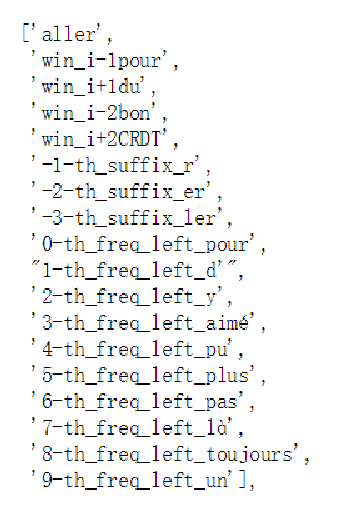
\includegraphics[scale=1]{featurealler.eps}
\caption{all feature values for word 'aller'}
\label{figure1}
\end{figure}

\subsection{Notion of Multiple Class and Perceptron}
$\bullet$ Each observation $x$ is associated to a label $y \in \YY$ where $\YY = $ finite set of all possible labels in train set. 

$\bullet$ Then we define the $0/1$ loss for the multi-class loss : 

\begin{equation}
\l^{multi}(y_1, y_2) = \left\{
\begin{aligned}
0 & & if\ y_1 == y_2\\
1 & &otherwise
\end{aligned}
\right.
\end{equation}

$\bullet$ Decision function. The most common we do is to use one weight vector $u_y$ for each label $y$. By this we get the decision function :

\begin{equation}
y^* = argmax_{y \in \YY} (x*u_y)
\end{equation}

We multiple the observation $x$ with each weight vector $u_y$ of each label $y$, and then we choose the label $y$ which gives the largest product. However, if we use one-hot encoding for the features mentioned above, the feature matrix will be very sparse (too many 0 and little 1), this will take many memories and it's not easy to train the model.

\textbf{For Perceptron : } So here we use the features encoded mentioned in \textbf{3.1}. And each feature value gets its own weight vector with one weight for each possible label. Figure \ref{figure2} is the weights for feature value 'win\_i-1pour', in which the feature name is 'win\_i-1' and the value for a word is 'pour'. In the figure, all possible labels associated with feature value 'win\_i-1pour' have a weight, some labels which are not in the dictionary have the weight value 0.

%the photo of weights
\begin{figure}[ht]
\centering
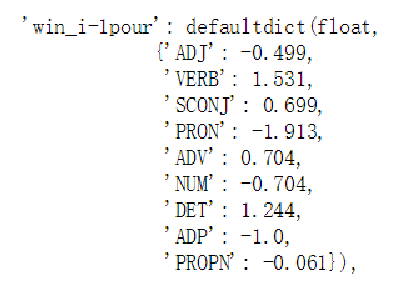
\includegraphics[scale=1]{weightpour.eps}
\caption{weights of feature 'win\_i-1pour'}
\label{figure2}
\end{figure}

We suppose $U$ as the dictionary of weights for all feature values $FV$,  for word $w_i$, we can get all the feature values $FV_i$. For each feature value $fv \in FV_i$, we can get the weight vector $u_{fv} = U[fv]$, in which, for each label $y \in \YY$ associated with a weight $u_y = u_{fv} [y]$. The decision function will be:

\begin{equation}
y^* = argmax_{y \in \YY} \sum_{fv \in FV_i} {u_{fv}[y]}
= argmax_{y \in \YY} \sum_{fv \in FV_i} {U[fv][y]}
\end{equation}

$\bullet$ Update rule. If $\l^{multi}(y^*, truth) = 0$ then we do nothing and if $\l^{multi}(y^*, truth) = 1$ then for each feature value $fv \in FV_i$ update the weights:

\begin{equation}
\forall fv \in FV_i,\  U[fv][y^*]\ -= 1;\ U[fv][truth]\ += 1
\end{equation} 

$\bullet$ Training and Testing. We use the same feature extraction in the train set of a corpus (not all corpus) and the same decision function as the training mentioned before. However, the difference between training and testing is that in training we find the prediction is not correct, then we use the updated rule to update the weights for reducing the loss, but when we are testing, we return the prediction predicted by the model and do nothing about the update.

\section{HMM}
Just as tomorrow's weather condition has a probability to be influenced by today's weather condition, the PoS tag of word also has a probability to be influenced by the PoS tag of last word. 
In this project, the state-of-the-art statistical tagger is trained : Hidden Markov Model (HMM) tagger \cite{charniak1993equations}.

\subsection{Notation}

Giving a sentence of words $W = (w_i,\dots,w_i,\dots,w_n)$, we aim to find a chain of labels (tags) $Y = (y_1,\dots,y_i,\dots,y_n)$, with each $y_i$ associated with a word $w_i$, which can maximiser $P(Y|W)$ : $Y^* = \mathop{\arg\max}_{Y} P(Y|W)$. According to Bayesian formula, $Y^* = \mathop{\arg\max}_{Y} P(W|Y)*P(Y)$. The HMM model will make predictions according to formula :

\begin{equation}
Y^* = \mathop{\arg\max}_{Y, y_i \in Y, w_i \in W} \prod_{i=1}^n P(w_i|y_i)*P(y_i|y_{i-1})
\label{hmm_formula}
\end{equation}

In the formula, $P(w_i|y_i)$ shows that the word $w_i$ present depends on the its possible associated label.$P(y_i|y_{i-1})$ shows that the current label type depends on which its last label was.\label{hmm notation}

\subsection{HMM tagger}
In this project we use the HiddenMarkovModel in the Pomegranate library to build a hidden Markov model for the PoS tagging. The steps for building HMM tagger as following:

\textbf{The state.} Supposing $\WW$ as the set of all possible word in the train set and $\YY$ as the set of all possible labels in train set. Each hidden state $y \in \YY$ gives the conditional probability $P(w|y)$ of observing a given word $w \in \WW$. The emission distribution for the word $w$ of the state $y$ is : $$P(w|y) = \frac{Count(y,w)}{Count(y)}$$ where $Count(y,w)$ is the number of pair of word $w$ and its label $y$, $Count(y)$ is the number of appearance of label $y$.

\textbf{The start and end transition.} We also have to estimate the starting probability distribution (the probability of each label being the first label of a sentence) and the ending probability distribution (the probability of each label being the last label of a sentence) from the train set : $$P(y|start) = \frac{Count(start, y)}{Count(start)}$$ 
$$P(y|end) = \frac{Count(end, y)}{Count(end)}$$ where $Count(start, y)$ is the number of the label y being the start of a sentence and $Count(start)$ is the number of sentences, similar in the case of end.

\textbf{The transition between two state.}The transition probability $P(y_i|y_{i-1})$ gives a the conditional probability of transition from label $y_{i-1}$ to $y_i$. From the train set we can learn the probabilities of all transitions from all state $y_i \in \YY$ to each state $y_j$ :
$$P(y_j|y_i) = \frac{Count(y_i, y_j)}{Count(y_i)}$$ where $Count(y_i, y_j)$ is count of pair $(y_i, y_j)$.

$\bullet$ Training and Prediction. We estimate all the terms $P(w|y)$, $P(y|start)$, $P(y|end)$, $P(y_j|y_i)$ based on a training corpus which is a set of couples $(W, Y)$ but not from all the corpus. We don't use any data in the test set. After all the terms estimated, we build the HiddenMarkovModel by adding all the states and transition mentioned before, and finally we use the model built to predict a sentence of labels for a sentence of input words.



\section{Evaluation}
The experimental results of Classifier Perceptron and HMM in the six corpus are presented in the Table 3 . The precision over the whole test set (i.e. the percentage of labels that have been correctly predicted) is presented in the column 'ALL'. The precision over the ambiguous words (i.e. the precision computed only on words that appear with more than one label in the train set) is presented in the column 'Ambiguous'. And the precision over OOV is presented in the column 'OOV'


\begin{table}[h]
\caption{The results}
\vspace{5pt}
\centering
    
\begin{tabular}{|l|rrr|rrr|}
\hline
\multicolumn{1}{|c|}{\ } & \multicolumn{3}{c|}{Perceptron} & \multicolumn{3}{c|}{HMM}\\ 
\cline{2-7}
Corpus & ALL & Ambiguous & OOV & ALL & Ambiguous & OOV\\
\hline
fr.ftb     & \textbf{95.53\%} & 95.14\% & \textbf{82.87\%} & \textbf{94.60\%} & 92.93\% & 48.24\% \\
fr.gsd     & 94.85\% & \textbf{95.61}\% & 81.84\% & 92.51\% & 93.82\% & 46.67\% \\
fr.partut  & 92.36\% & 89.66\% & 72.72\% & 91.73\% & 91.90\% & 53.26\% \\
fr.pud     & 84.43\% & 93.44\% & 67.60\% & 77.68\% & 91.90\% & 51.87\% \\
fr.sequoia & 92.61\% & 91.64\% & 75.19\% & 93.73\% & \textbf{94.22\%} & \textbf{57.82\%} \\
fr.spoken  & 89.23\% & 90.97\% & 78.57\% & 86.54\% & 90.34\% & 51.10\% \\
\hline
\end{tabular}
\label{results}
\end{table}


\subsection{For Perceptron}
We trained the Perceptron classifier on the training set. A word in the test set is classified by Perceptron by  building the feature values using the same extraction of features as the train set. 


$\bullet$ For ALL. From the results of precisions on ALL on all the corpus (Table \ref{results}) we can get that the perceptron has a maximum precision at 95.53\% on the corpus 'fr.ftb', and then 95.85\% on 'fr.gsd'. The precisions on the others are less accurate because the corpus 'fr.ftb' and 'fr.gsd' has much larger train data set than others (Table \ref{test_on_train}) and this gives much more training on the Perceptron, another reason is that the two corpus have a less value of KL (Table \ref{table_matric}) which means their test set has a larger similarity with the train set. For the corpus 'fr.pus', it doesn't have many train data set, but more test data set than train data set (103\% on Table \ref{test_on_train}) and it has largest value of KL.

\begin{table}[h]
\caption{test words}
\vspace{5pt}
\centering
\begin{tabular}{|c|r|r|r|r|r|r|}
\hline
\ & fr.ftb & fr.gsd & fr.partut & fr.pud & fr.sequoia & fr.spoken \\
\hline
Test words & 75073 & 9742 & 2515 & 24138 & 9740 & 10010 \\
\hline
Train words & 442228 & 345009 & 23324 & 23324 & 49173 & 14952 \\
\hline
Rest/Train & 17\% & 2\% & 11\% & 103\% & 20\% & 67\%\\  
\hline
\end{tabular}
\label{test_on_train}
\end{table}


$\bullet$ For OOV. We get that the two corpus ('fr.frb \& fr.gsd') have the largest precision, the reason is similar with previous precisions on ALL : much larger train data set. But for 'fr.pud', it has only 67.60\% on OOV, this is because the largest number of OOV words (6540, Table \ref{table_matric}) and largest percentage of OOV words on test set (72.56\%, Table  \ref{table_matric}). The Perceptron doesn't have the power to get good precision on large percentage unknown words test data set but small train data set size. However, for the corpus 'fr.spoken', it has larger precision (78.57\%) compared to 'fr.pud' although it has almost the same large percentage of OOV (60.51\%). The reason is that 'fr.spoken' comes from spoken french (Table \ref{table_resource}), and the distribution feature works better on the corpus which has less normative expression.. 

$\bullet$ For Ambiguous Words. We get that the two corpus ('fr.frb \& fr.gsd') have the largest precision, but the precision on other corpus is similar with them except 'fr.partut'. The reason is that 'fr.partut' is consisted of a variety of text genres, including talks, legal texts etc. As a consequence, its composition is too messy to get a good precision on Ambiguous words.



\begin{table}[h]
\caption{Ambiguous words}
\vspace{5pt}
\centering
\begin{tabular}{|c|r|r|r|r|r|r|}
\hline
\ & fr.ftb & fr.gsd & fr.partut & fr.pud & fr.sequoia & fr.spoken \\
\hline
Ambiguous words & 212787 & 151557 & 7243 & 7243 & 16096 & 4151 \\
\hline
Total train words & 442228 & 345009 & 23324 & 23324 & 49173 & 14952 \\
\hline
Ambi/Total & 48\% & 44\% & 31\% & 31\% & 33\% & 28\%\\  
\hline
\end{tabular}
\end{table}

\subsection{For HMM}  

$\bullet$ For ALL and Ambiguous. HMM tagger gets almost the same results as Perceptron (Table \ref{results}) except the precision on 'fr.spoken' over ALL, because for HMM tagger the current label type depends on which its last label was (\ref{hmm notation}), but the 'fr.spoken' has much normative expressions which make HMM tagger work worse on 'fr.spoken' than on the others. And there exist many errors for the verbs 'etre' and 'avoir' between tag auxiliary and verb.

$\bullet$ For OOV. HMM tagger works much worse than Perceptron over OOV(Table \ref{results}). The reason is that according to Formula \ref{hmm_formula}, $P(w_i|y_i)$ is estimated by the train set, but one word of oov $\forall w_{oov} \in OOV$ doesn't exist in train set, so when we are in prediction, $P(w_{oov}|y_i)\ will\ be\ 0$ which results that $\prod_{i=1}^n P(w_i|y_i)*P(y_i|y_{i-1})$ will be 0, and the HMM will not work on OOV. However, in our experiment, we replaced the OOV words by 'nan', and then gave $ P(w_{nan}|y_i)$ a very small probability : $$\forall{y_i, w_{oov}}, y_i \in \YY, w_{oov}  \in OOV, P(w_{oov}|y_i) = P(w_{nan}|y_i) = p_{low}$$ where $w_{nan}$ is the word 'nan' and $p_{low} = a\ very\ small\ probability$. 

\section{Conclusion}
We have presented Perceptron and HMM tagger and all the work we have done.The resource of corpus, the noises of corpus can do influence to the results. In our experiment, Perceptron works better than HMM tagger, especially in OOV. However, HMM tagger has much more improvement can be done such as Treetagger\cite{schmid1994probabilistic}. The future work is to find more features for Perceptron and handle the problem of OOV. 

\bibliographystyle{plain} 
%\bibliographystyle{splncs} 
\bibliography{biblioML}

\end{document}
